\documentclass{article}

\usepackage{times}
\usepackage{graphicx}
\usepackage{subfigure}
\usepackage{natbib}
\usepackage{algorithm}
\usepackage{algorithmic}
\usepackage{todonotes}
\usepackage{float}
\usepackage{amsmath}
\usepackage{booktabs}
\usepackage{hyperref}
\usepackage{color,soul}
\usepackage{array}
\usepackage[accepted]{icml2017}

\newcommand{\hlc}[2][yellow]{{%
    \colorlet{foo}{#1}%
    \sethlcolor{foo}\hl{#2}}%
}

\icmltitlerunning{CS 287 Final Project}

\begin{document}

\twocolumn[
\icmltitle{Investigating Factual Accuracy in Abstractive Summarization Models}
\begin{icmlauthorlist}
\icmlauthor{Samuel Hsiang}{}
\icmlauthor{Celine Liang}{}
\end{icmlauthorlist}

\vskip 0.3in
]

\begin{abstract}
The task of summarization---condensing an input ``source document'' into a shorter ``output summary''---has long been an active area of research in Natural Language Processing. Though simple for humans, doing summarization \textit{accurately} has been somewhat of a challenge for neural models, as this involves locating, extracting, and conveying the most important pieces of information from the source document in a concise and accurate manner. The difficulty of this task is precisely what makes summarization so important, but modern machine summarization models have been known to misrepresent and fabricate facts that do not appear in the source documents, rendering outputted summaries unreliable and essentially useless. In this work, we analyze the outputs produced by these machine summarization models to determine the extent of their abilities (or lack thereof) to accurately convey information that we are confident was originally contained in the source documents.
\end{abstract}

\section{Introduction}
\label{sec:introduction}

% Example Structure:
% \begin{itemize}
% \item What is the problem of interest and what (high-level) are the current best methods for solving it?
% \item How do you plan to improve/understand/modify this or related methods?
% \item Preview your research process, list the contributions you made, and summarize your experimental findings.
% \end{itemize}

Machine summarization has been an active area of research in Natural Language Processing for quite some time. The task of summarization, though simple for humans, has been somewhat of a challenge for neural models; one of the most difficult aspects is how to locate, extract, and then convey the most important pieces of information from the source document in a concise and accurate manner. The difficulty of this task is precisely what makes summarization so important, but output summaries are only practical and useful if they do not contain inaccurate facts or contradictions to the source document. 

Modern machine summarization models attempt to learn to produce factually correct outputs but are still prone to factual inaccuracies and misconveying information. The current standard for evaluating the score of a summarization model, the ROUGE metric, measures the n-gram overlap with the reference summary \cite{lin2004rouge}. This is useful as a first order approximation for the effectiveness of the summarization model but there is evidence that many state-of-the-art summarization models, though high in ROUGE score, do not produce factually accurate summaries. In particular we note that switching the subject and object of a sentence minimally effects the ROUGE score but causes the new sentence to claim something that is factually incorrect.

In this work, we investigate this problem further, and develop a method for identifying and flagging abstractive summaries that make false claims not supported by the source document. To our knowledge, no previous works have undertaken this type of analysis, though many have developed models that they claim to increase the facutal accuracy of the generated outputs. The goal of this work is to evaluate and analyze the factual accuracy of outputs generated by abstractive summarization models. We use a dependency parser to extract important relations pertaining to the source document and the generated summary, then compare these relations with relevant relations from the source document to determine the extent to which the generated summary remains faithful to the source document.
% We focus on 3 abstractive summarization models: the Pointer-Generator model \cite{see2017get}, the Bottom-Up Abstractive Summarization model \cite{gehrmann2018bottom}, and Fast Abstractive Summarization with Reinforce-selected Sentence Rewriting \cite{chen2018fast}.
We focus on two abstractive summarization models: the Pointer-Generator model \cite{see2017get} and the Bottom-Up Abstractive Summarization model \cite{gehrmann2018bottom}.
Our code can be found \href{https://github.com/alwayswimmin/cs287-f}{here}.

\section{Background}
\label{sec:background}

% Example Structure:
% \begin{itemize}
% \item What information does a non-expert need to know about the problem domain?
% \item What data exists for this problem?
% \item What are the challenges/opportunities inherent to the data? (High dimensional, sparse, missing data, noise, structure, discrete/continuous, etc?)
% \end{itemize}

The task of summarization can be described as the following: given a source document of tokens $x_1, x_2, x_3 \dots, x_n$, produce a shorter sequence of tokens $y_1, y_2, \dots, y_n$ that captures the meaning of the original source. In machine summarization, models can generally be divided into two classes: \textit{extractive} models, which build summaries by directly extracting sentences or phrases from the original source, and \textit{abstractive} models, which generate words for the summary output without being restricted to the exact phrasing of the original source. Since extractive models directly extract sentences from the source document, the likelihood of misconveying the information that was originally intended by the source is fairly low. Conversely, abstractive models generate words for the output based on the original document but may not necessarily adhere to the original wording; this leaves room for fabrication which leads to factual inaccuracies. 

The metric which has become the standard for evaluating the accuracy of machine summarization models, the ROUGE metric, does not directly capture the factual accuracy of a summary, and instead only measures the n-gram overlap with a reference summary. Specifically, ROUGE-n is the n-gram recall between a candidate summary $S_{\text{cand}}$ and a set of reference summaries $S_{\text{ref}}$ (often containing just one reference summary), computed as
$$\text{ROUGE-n}(S_{\text{cand}}) = \frac{\sum \limits_{S \in S_{\text{ref}}} \sum \limits_{x_i \in S} N(x_i, S_{\text{cand}})}{\sum \limits_{S \in S_{\text{ref}}} \sum \limits_{x_i \in S} N(x_i, S)}$$
where $n$ is the length of the n-gram, $x_i$ is the $i^{th}$ n-gram in summary $S$, $N(x_i, S_{\text{cand}})$ is the number of times n-gram $x_i$ appears in the candidate summary $S_{\text{cand}}$, and $N(x_i, S)$ is the number of times n-gram $x_i$ appears in the reference summary $S$ \cite{lin2004rouge}. The ROUGE metric is a useful first-order measure of the effectiveness of machine-generated summary but does not measure how well the summary represents the factual information of the original document. More importantly, it is unknown to what extent current state-of-the-art that achieve high ROUGE scores are able to produce factually accurate summaries.

Rather than using ROUGE to measure the score of a summary, we turn to sentence structure to extract the basic facts that are represented in each sentence of a summary. The main challenge in measuring factual accuracy, is determining \textit{equivalency}, i.e. if two sentences (or phrases) convey the same meaning. Our approach breaks down the sentences outputted by an abstractive summarization model using a neural dependency parser that has been trained to learn syntactical relationships of words within a sentence. We discuss our use of syntax further in Sec. \ref{sec:methods}. 

The main source of data that is used in this work (and also in the models we consider) is the CNN/Daily Mail data set. CNN/Daily Mail is a collection of news articles from the CNN and Daily Mail newspapers, which are used as source documents, and the first three bullets of human-written summaries corresponding to each article, which are used as reference (or target) summaries. Because of the bullet point format, the ``summaries'' that are learned by the abstractive summarization models that we are analyzing sometimes do not take the form of complete sentences; this is somewhat problematic for our dependency parser, which assumes the syntax of a complete sentence, but we simply choose to ignore those outputs of the dependency parser which are sometimes incorrect.
\section{Related Work}
\label{sec:related}
% Example Structure:
% \begin{itemize}
% \item What 3-5 papers have been published in this space?
% \item How do these  differ from your approach?
% \item What data or methodologies do each of these works use?
% \item How do you plan to compare to these methods?
% \end{itemize}

Current state-of-the-art abstractive summarization models, while able to achieve high ROUGE scores, have been known to misconvey the facts of the source document. Therefore, in order for the task of neural summarization to be possible for actual use, the issue of factual accuracy in abstractive summarization models is quite a pressing one. While many previously proposed methods claim to improve the factual accuracy of abstractive summarization models, there has not yet been any research done to directly analyze the outputs of these models to gauge whether or not these claims are true. We discuss these models in further detail below, noting that all were trained using the CNN/Daily Mail data set which we described earlier.

The first well-known work which proposed a method claiming to address the issue of factual accuracy was the Pointer-Generator model. Part of the appeal of the Pointer-Generator model was that it learned to directly copy from the source document, which the authors claimed led to higher factual accuracy and less fabrication \cite{see2017get}. The drawback was that this model tended to copy long strings of words directly from the source document, reducing the benefit of ``summarizing'' the document. 

To address the problem of copying long strings of words from the source, a two-step ``Bottom-Up'' abstractive model was proposed by Gehrmann et al. to first select content then either copy, or generate, relevant words; they also impose a coverage penalty to constrain the length of the phrase that can be copied \cite{gehrmann2018bottom}. % Another model, from the paper ``Fast Abstractive Summarization with Reinforce-Selected Sentence Rewriting'', works similarly to the Bottom-Up model, but on the sentence granularity; it first extracts sentences from the source document, using reinforcement learning to maximize the ROUGE score of these extracted sentences using the REINFORCE policy gradient algorithm, then abstractly rewrites these extracted sentences \cite{chen2018fast}. 

We focus on the two works we mention above in our analysis to determine the extent that the respective copy mechanisms are successful in remaining faithful to the sources, and the extent to which the ``abstractive'' portions lead to fabrication. These two works also have generated outputs that are readily available on their GitHubs. 

Other works have tried to incorporate mechanisms to infuse factual accuracy directly into the model. One such work, which partially motivated our use of the dependency parser, uses the dependency parser to extract important dependencies from the source document, encodes both the source document and the important dependencies using a dual-attention encoder, and then combines the encoder outputs for decoding as in the standard seq2seq model \cite{cao2018faithful}. Another work uses multitask learning on the decoder of a seq2seq to learn both the task of summarization and the task of entailment generation from Natural Language Inference, claiming that the NLI task improves the logical flow (entailment) in the decoded summary \cite{pasunuru2017towards}. Both \cite{pasunuru2017towards} and \cite{cao2018faithful} train on the Gigaword corpus, which is a collection of news articles, used as sources, and their respective headlines, used as summaries. Because of the ``headline'' nature of the generated summaries, they often do not form complete sentences and are more difficult to analyze; for this reason, we do not focus on these particular works.

% \todo[inline]{took out Models and Inference section, idk if we want to add later}
% \section{Models}

% Example Structure:

% \begin{itemize}
% \item What is the formal definition of your problem?
% \item What is the precise mathematical model you are using to represent it? In almost all cases this will use the probabilistic language from class, e.g.
%   \begin{equation}
%   z \sim {\cal N}(0, \sigma^2)\label{eq:1}
% \end{equation}
% But it may also be a neural network, or a non-probabilistic loss,
% \[ h_t \gets \mathrm{RNN}(x_{t}, h_{t-1} )\]

% This is also a good place to reference a diagram such as Figure~\ref{fig:diagram}.

% \item What are the parameters or latent variables of this model that you plan on estimating or inferring? Be explicit. How many are there? Which are you assuming are given? How do these relate to the original problem description?
% \end{itemize}

% \begin{figure}
%   \centering
%   \missingfigure[figheight=8cm]{}
%   \caption{\label{fig:diagram} This is a good place to include a diagram showing how your model works. Examples include a graphical model or a neural network block diagram.}
% \end{figure}

% \section{Inference (or Training)}

% \begin{itemize}
% \item How do you plan on training your parameters / inferring the
%   states of your latent variables (MLE / MAP / Backprop / VI / EM / BP / ...)

% \item What are the assumptions implicit in this technique? Is it an approximation or exact? If it is an approximation what bound does it optimize?

% \item What is the explicit method / algorithm that you derive for learning these parameters?
% \end{itemize}

% \begin{algorithm}
%   \begin{algorithmic}
%     \STATE{\lipsum[1]}
%   \end{algorithmic}
%   \caption{Your Pseudocode}
% \end{algorithm}

\section{Methods}
\label{sec:methods}
% \begin{itemize}
% \item What are the exact details of the dataset that you used? (Number of data points / standard or non-standard / synthetic or real / exact form of the data)

% \item What are the exact details of the features you computed?


% \item How did you train or run inference? (Optimization method / hyperparameter settings / amount of time ran / what did you implement versus borrow / how were baselines computed).

% \item What are the exact details of the metric used?
% \end{itemize}

% Problem Definition
% Relation: Actor, Action, Acted Definition
% Dependency Parser Motivation
% From Dependency Parser to Actor, Action, Acted
% BERT Natural Language Inference Integration
% Error Types

As stated previously, we focus on analyzing two related models: the original Pointer-Generator model \cite{see2017get} and Bottom-Up Abstractive Summarization \cite{gehrmann2018bottom}. %, and Fast Abstractive Summarization with Reinforce-Selected Sentence Rewriting \cite{chen2018fast}. 
Our methods are highly motivated by techniques from \cite{pasunuru2017towards} and \cite{cao2018faithful} but rather than incorporating them into a model, we explicitly apply them to analyzing containment of factual information. We use a dependency parser to extract ``important'' dependencies, which we will define in a later subsection, and use BERT \cite{devlin2018bert} finetuned on the task of Natural Language Inference to determine if two sentences can be considered semantically equivalent. We also use a neural coreferencing system to carry out coreference resolution.

For the dependency parser, we utilize the \textit{spaCy} package \cite{spacy2}, which can be found \href{https://spaCy.io/usage/linguistic-features}{here}. Our BERT implementation is derived from Dong-Hyun Lee's \href{https://github.com/dhlee347/pytorchic-bert}{pytorchic-bert} which is in turn based off of HuggingFace's \href{https://github.com/huggingface/pytorch-pretrained-BERT}{implementation} \cite{neuralcoref}. We use a pretrained BERT-base finetuned on the MNLI dataset for Natural Language Inference. For the neural coreferencing system, we use an implementation by HuggingFace, which can be found \href{https://github.com/huggingface/neuralcoref}{here}.

\subsection{Problem Specification and Definitions}

We restrict the notion of factual accuracy to only consider what we define as \textit{relations}, which encapsulate ``facts'' described in a document. A relation consists of a verb, which we define as the \textit{action}, and the ``doers'' and ``receivers'' of that action, which we define as \textit{actors} and \textit{acteds} respectively.  We denote a relation $R$ as the tuple $(action,\{actors\},\{acteds\})$. For example, in the sentence ``Alice and Bob moved the table," ``Alice" and ``Bob" are the actors, ``moved" is the action, and ``table" is the acted, which produce the relation (moved, \{Alice, Bob\}, \{table\}).

A relation $R_S = (V_S,\mathcal{A}_S,\mathcal{B}_S)$ in the summary is defined as \textit{implied} by another relation $R_D = (V_D,\mathcal{A}_D,\mathcal{B}_D)$ if their respective actions $V_R \equiv V_D$ are equivalent (where equivalency is define in later subsections) and the actor and acted sets are contained $\mathcal{A}_S \subseteq \mathcal{A}_D, \mathcal{B}_S \subseteq \mathcal{B}_D$, again allowing for equivalency. For example, if the source document contains the sentence ``Alice and Bob after some deliberation moved the chairs and the table," then the relation (moved, \{Alice, Bob\}, \{chairs, table\}) implies the first relation described above. A relation that is implied by some relation in the source document is \textit{attested} by the document.

\subsubsection{Scope and Motivation}

The primary goal of this project is to determine whether each $(action, actor, acted)$ tuple in the summary is attested by the document. At first glance, this can simply be found by checking whether a summary relation is contained in the set of document relations---and this motivates our decision to use the Pointer-Generator and Bottom-Up models since most words in the generated outputs are directly copied from the source. However, there are more nuances to take into consideration. For instance, if two \textit{actors} (or \textit{acteds}) can be shown to be the same entity, e.g. a pronoun substituted for its antecedent, then the summary relation should be considered to follow from the document relation, even though direct containment does not hold. Furthermore, two actions can loosely be considered equivalent if the verbs' underlying lemmas are considered equivalent, even if tense is different. (Strictly speaking, this may not be completely factually correct, but we decided to allow for tense differences.) However, a direct object attributed to different verbs in the document and the summary should be identified as a potential error.

\subsection{Tools}

\subsubsection{Dependency Parser}

The main tool that we use is the dependency parser, which extracts syntactical dependencies (as well as the corresponding labels \textit{nominative subject}, \textit{direct object}, etc.) that we then use to construct our relations. Technically, we wish to determine \textit{semantic} equivalency of relations, whereas the dependency parser extracts \textit{syntactical} relationships; however, we disregard this difference, as we view our decision to use the dependency parser as the most reasonable proxy for evaluating factual accuracy at the granularity that we desire. But we do not completely disregard semantic equivalency, and use the task of Natural Language Inference as a proxy for determining semantic equivalency when necessary. We start by applying the dependency parser to extract the syntactical relations that we are more confident of, and then use the strongest model we can find, BERT, to determine semantic equivalencies when necessary. We also note that the \textit{spaCy} dependency parser we have chosen to use is not perfect and sometimes mislabels dependencies. We discuss this further in Sec. \ref{sec:discussion}.

\subsubsection{BERT for Natural Language Inference}
In addition to using the dependency parser to extract relations, we also utilize a large language model, BERT, to determine semantic equivalencies \cite{devlin2018bert}. Specifically, we finetune  BERT-base on the Natural Language Inference dataset MNLI to get a model capable of classifying pairs of sentences as \textit{entailed}, \textit{neutral}, or \textit{contradiction}. The validation accuracy of this model on the MNLI dataset is $84.0\%$. We use BERT only in the cases where we are unable to find an exact verb match, which we will discuss below.

\subsubsection{Neural Coreferencing System}
We use Hugging Face's extension of \textit{spaCy} to find coreference clusters in our document. All pairs of noun phrases in a document are assigned coreference scores, and those noun phrases with coreference scores beyond a certain threshold are considered part of the same cluster. We use the default coreference greediness parameter of 0.5, and for each noun phrase in a cluster, we isolate the roots of the noun phrases, treating those nouns as referring to equivalent entities. We noticed this system tends to struggle with quotations and first person pronouns in quotations and discuss our workaround for this issue below.

% is still useful for supplementing action equivalencies in cases where simple cosine similarity between different verbs might fail. A concrete example of this is substituting ``said" for ``stated." Thus, when we can recognize that one relation would imply another but for action equivalency, i.e., the actors set and the acteds set are contained, we feed both sentences into a Natural Language Inference system to test whether one action could be inferred from another. We hypothesize that NLI integration is more useful when applied to verbs rather than nouns, as nouns, at least in our dataset, have less ambiguity in resolving the identity of an actor or agent, whereas whether or not an action follows from another is more loose; we therefore choose to apply NLI only to verb equivalency. We used BERT-base (\todo{describe and cite here?}) finetuned on the MNLI dataset for Natural Language Inference to accomplish this task.


\subsection{Extracting \textit{actors} and \textit{acteds} relations}

We design our classification primarily to detect incorrect relationships between verbs and their subjects and objects. For this reason, we focus on the dependencies nominative subject \textit{nsubj}, direct object \textit{dobj}, the passive nominative subject \textit{nsubjpass}, and the object of the preposition ``by''. A noun that is the \textit{nsubj} for a verb in the generated summary is expected to be attested as the actor for that verb in the source document. Likewise, a noun that is the \textit{dobj} is expected to be attested as the acted of that the action represented by that verb in the source document. In a sentence with passive voice, the subject \textit{nsubjpass} is actually the receiver of the action represented by the verb, and therefore the subject is added to the set of acteds for that verb. Similarly, the agent of a prepositional phrase beginning with ``by" is added to the set of actors for that verb. We capture participles that are labeled with the dependency \textit{acl}, where the noun being modified is appropriately labeled as an actor or an acted. For example, the phrase ``the 31-year-old, signed from Swansea in the summer" yields the acted ``old" for the action ``signed."

\subsection{Determining Equivalency}

Oftentimes, the summarization model chooses to replace a word from the original source document with another word that conveys the same meaning. We discuss our use of cosine similarity, coreferencing, and BERT to determine equivalency in the following sections.

\subsubsection{Noun equivalency}
Two nouns are said to be equivalent if the cosine similarity of the respective \textit{spaCy} word embedding vectors exceeds a certain threshold. We use noun similarity threshold $0.8$.

We additionally use relative clauses to establish equivalencies that can be inferred from the sentence's dependency structure. In the sentence ``the dog that caught the ball gave it to the man," ``that" is the \textit{nsubj} for ``caught" and the \textit{relcl} for the verb ``caught" is ``dog." Therefore, we recognize ``that" and ``dog" as referring to the same entity. 

However, using only these methods fail to take into account pronouns and their antecedents, or other types of word substitutions (e.g. substituting a person's full name with their first or last name). Therefore, we use a neural coreferencing system to identify equivalent entities both within a source document and within the generated summary. But, as mentioned above, the neural coreferencing system struggles with quotations and first person pronouns in quotations. To resolve this difficulty, we build our own quote speaker reference that identifies a speaker for each quote. For a block of text enclosed by quotes, we search for a word whose dependency is \textit{ccomp} and whose dependency head lies outside that quote block. In most cases the dependency head is a verb such as ``said" or ``stated." Then an actor for that verb is considered equivalent to first person pronouns within the quotation.

\subsubsection{Verb Equivalency}
We consider to be equivalent any verbs with the same underlying lemma. Similar to our method of determining noun equivalency, we also use the cosine similarity of the \textit{spaCy} word embeddings, with a verb similarity threshold of $0.9$, to determine if two verbs are equivalent. In the cases where we have found dependencies with satisfactory actors and acteds, but the verbs do not meet the cosine similarity threshold, we use our finetuned BERT NLI model to determine if the sentences corresponding to two relations with equivalent actors and acteds are ``entailed'', or essentially if they have similar verbs.

\subsection{Error Classification}
\label{sec:classification-type}

Beyond simply listing whether a relation is attested in the source document or not, we also provide an attempt to classify the type of error being made. The classes we have defined, in the order of precedence in classification, is as follows:
\begin{enumerate}
    \item Containment: A relation in the summary is implied by a relation in the source document by direct containment.
    \item Contradiction: Given a relation in the summary, a relation in the source document is found where the actor (or acted) is found in the acted (or actor) position, i.e. the ``doer'' and receiver'' of a relation is flipped.
    \item Invalid simplification: Given a relation in the summary, a relation in the source document is found containing one half of the relation (the action and actors), and a separate relation is found containing the other half (the action and acteds), but because these are separate relations in the source document, they do not jointly imply the queried relation.
    \item Missing actors/acteds: Given a  relation in the summary, a relation in the source document is found containing the action and acted but not the actor, or containing the action and actor but not the acted.
    \item Entailed verb (BERT): A relation is implied by the source document when allowing dissimilar verbs to be resolved by BERT NLI.
    \item Contradictory verb (BERT): A relation with a contradictory verb, as determined by BERT NLI, is found in the source document.
    \item Missing verb (BERT): A relation containing the actors and acteds but with a different action is found in the source document. This occurs when BERT does not classify the verb as entailed or contradictory, and instead outputs a neutral classification.
    \item Missing dependencies: the default fallback, where the missing dependency could not be more finely classified.
\end{enumerate}

Once again, we note that BERT NLI is only used for summary relations with actors and acteds that are contained in a source relation but whose corresponding verbs are below the verb similarity threshold. The relation must satisfy containment of actors and acteds in a source sentence relation, but have dissimilar verbs.
% the dependency parser we are using tends to have errors which we hope to catch with BERT NLI. this does not always work, as we discuss further in Sec. \ref{sec:discussion}.

\subsection{Average Copy Length}
\label{copy-length}
To help analyze generated summaries, we define \textit{average copy length} for a summary. For a word $w$, its \textit{word copy length} $l(w) = \max \{l : \exists i,j : w \in S_{i:i+l} = D_{j:j+l} \}$ is the length of the longest contiguous subsequence of tokens containing $w$ shared by both the source document $D$ and the generated summary $S$. The \textit{average copy length} is defined as the average $\frac{1}{|S|} \sum_{w\in S} l(w)$ of the word copy lengths over all token in the summary. In the case where copy sequences do not overlap, this is equivalent to taking a weighted average of the copy length of all copy sequences.

\pagebreak
\section{Results}
\label{sec:results}
% \begin{itemize}
% \item What were the results comparing previous work / baseline systems / your systems on the main task?
% \item What were the secondary results comparing the variants of your system?
% \item This section should be fact based and relatively dry. What happened, what was significant?
% \end{itemize}
First, we note that the Pointer-Generator model (with coverage) that we are analyzing achieved ROUGE-1, ROUGE-2, and ROUGE-L scores of 39.53, 17.28, and 36.38. The Bottom-Up Abstractive Summarization model achieved higher ROUGE scores of 41.22, 18.68, and 38.34. In our analysis, we use 7000 randomly chosen examples from the CNN/Daily Mail in our calculations and plots.

Table \ref{fig:summary} shows a summary of the distribution of the errors classified by our model. The numbers in parentheses denote the corresponding number when taking into account BERT-based evaluations, assuming that relations with verbs that are considered entailed by BERT are contained, and relations that are considered contradictions by BERT are contradictions. We note that the Pointer-Generator model produces significantly more summaries with $100\%$ contained relations (completely factually accurate by our metric) than the Bottom-Up model, as well as fewer summaries containing at least one contradictory relation.

\begin{table}[H]
  \centering
  \begin{tabular}{m{10em}||m{5em}|m{5em}}
  & Bottom-Up & Pointer-Generator \\
  \hline
$100\%$ containment & 2343 (2436) & 4696 (4750)  \\
\hline
Contains contradiction & 575 (699) & 284 (294) \\
\hline
Other & 4082 (3865) & 2020 (1956) \\
\hline
Total & 7000 & 7000
\end{tabular}
 \caption{Factual Accuracy Statistics}
  \label{fig:summary}
\end{table}

Taking the BERT-based evaluations as correct, we find that the Pointer-Generator model achieves a perfectly factual summary $67.86\%$ of the time while the Bottom-Up Abstractive Summarization model achieves perfect factual accuracy of $34.80\%$ of the time, indicating that the Pointer-Generator model contains more perfectly factual summaries.

We also calculate average copy length corresponding to each summary outputted by both models. A comparison of the distributions of average copy length of summaries is shown in Figure \ref{fig:all_hists}. The Bottom-Up model copies $14.9$ words on average, while the Pointer-Generator model copies $27.58$ words on average. Also pictured is the distribution over summaries of the fraction of relations in the summary that is contained in the source, and the distribution of the fraction of contradictory relations for summaries with at least one contradictory relation.

\begin{figure*}
  \centering
  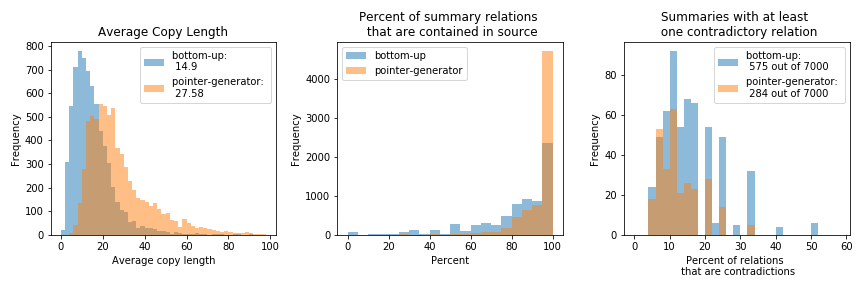
\includegraphics[width=\linewidth]{figs/all_hists.png}
  \caption{Comparison of Bottom-Up and Pointer-Generator}
  \label{fig:all_hists}
\end{figure*}

\subsection{Error Classification Across Models}

We also note the average fraction of relations that are flagged as having missing actors and acteds for both the Bottom-Up and Pointer-Generator models. These percentages are shown in Table \ref{fig:missing}.

\begin{table}[H]
  \centering
  \begin{tabular}{m{8em}||m{5em}|m{5em}}
  & Bottom-Up & Pointer-Generator \\
  \hline
Missing actors & 7.09\% & 2.61\%  \\
\hline
Missing acteds & 4.15\% & 1.30\% \\
\hline
Other Missing & 2.49\% & 0.17\% \\
\hline
Total Percentage of Missing Relations & 13.74\% & 4.08\% 
\end{tabular}
 \caption{Factual Accuracy Statistics}
  \label{fig:missing}
\end{table}

As expected, we notice that there are fewer missing relations in summaries produced by the Pointer-Generator model than the more abstractive Bottom-Up model.

Finally, Figure \ref{fig:contradictions} compares the percent of contradictory relations found in those summaries with at least one relation found to be a contradiction (including our BERT-based evaluations) with the corresponding average copy length and ROUGE-1 score. The left plot, which plots average copy length against the percent of relations for each summary flagged to be contradictions, shows a strong negative correlation for both models indicating that summaries with shorter strings of copied words have higher fractions of contradictory relations. The right plot, which plots ROUGE-1 score against the percent of relations for each summary flagged to be contradictions, has no clear correlation. From these plots we are able to visualize the drawback of the ROUGE-1 metric which simply calculates n-gram overlaps with no regard to factual information.

\begin{figure}
  \centering
  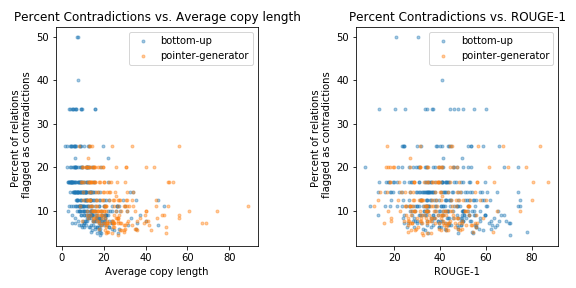
\includegraphics[width=\linewidth]{figs/contradictions-bu-pg.png}
  \caption{Contradictions vs. Copy Length (left). Contradictions vs. ROUGE-1 (right)}
  \label{fig:contradictions}
\end{figure}


% \begin{table}
%   \centering
%   \missingfigure[figheight=5cm]{}
%   \caption{Secondary table or figure in results section.}
%   \label{fig:mainres}
% \end{table}

\subsection{System Accuracy: Manual Verification}

By manually verifying our system's analysis of 20 random outputs from both Bottom-Up and Pointer-Generator (see appendix \ref{sec:manual-verification}), we can check our system's accuracy when it flags something as incorrect vs. correct, where a relation is marked as ``correct" if it is labeled as contained or entailed from BERT and ``incorrect" otherwise.

Of the 335 times our system marked a relation as correct, we determined that this was accurate 331 times, and we determined that the relation's factuality was questionable 4 times. We determined that for each of the questionable relations, it was still conceivable that the relation might follow logically, but the relation might not necessarily follow from our system specification.

Of the 46 times our system marked a relation as incorrect, we determined that this was accurate 20 times, questionable 6 times, and verifiably inaccurate 20 times. However, among the 20 verifiably inaccurate relation classifications, 15 can be further classified into one of three main problem areas (coreferencing, summary punctuation, and conjunction) such that improvements in any of these submodules along the pipeline would have caught these errors. We explore this further in the discussion.

\section{Discussion}
\label{sec:discussion}

% \begin{itemize}
% \item What conclusions can you draw from the results section?
% \item Is there further analysis you can do into the results of the system? Here is a good place to include visualizations, graphs, qualitative analysis of your results.
% \item  What questions remain open? What did you think might work, but did not?
% \end{itemize}

We refer to appendix \ref{sec:examples} for specific elucidating examples of instances of errors that our model was (and was not) able to classify. The appendix contains examples of the particular classification types described in \ref{sec:classification-type}. In this section we will discuss trends that we have noticed across examples from our manual verification and from our analysis of our plots.

\subsection{General Trends}

As expected, because the Pointer-Generator model copies sequences at longer lengths at a time than Bottom-Up Summarization, it attains perfect factual accuracy as measured by our system at significantly higher frequencies than Bottom-Up Summarization. We see from figure \ref{fig:contradictions} that contradictions tend to be negatively correlated with copy length but does not seem to be correlated with ROUGE, which means that even though Bottom-Up Summarization outperforms Pointer-Generator in ROUGE, its worse performance according to our factual accuracy metric indicates that ROUGE probably should not be the sole metric by which to judge summarization models.

\subsection{Analyzing Incorrectly Classified Errors}

\subsubsection{Accuracy Between Models}

Of course, our factual accuracy metric is not useful in making relative judgements between the performance of two models if it is less precise for one model than the other. Indeed, it is conceivable that as a model becomes more abstractive, our fact-checking system becomes less accurate. However, from our manual verification from appendix \ref{sec:manual-verification}, we see that of the 11 times we flag a relation from Pointer-Generator as incorrect, 7 times were inaccurate, and the relation was actually factually accurate, while for Bottom-Up Summarization, of the 35 times we flag a relation as incorrect, 13 times our system was mistaken. So, it seems that our system actually is more prone to mistakenly labeling a relation as not factual for Pointer-Generator than for Bottom-Up Abstractive Summarization, so our conclusions from the discussion above probably still hold.

\subsubsection{Coreferencing}

From the 20 verifiably inaccurate relation classifications, we found that 11 of these were due to poor coreferencing: we found that most of our errors corresponding to falsely flagging a true statement as incorrect were due to the coreference system failing to detect that two entities are equivalent. We encountered the following common mistake where a relation with a pronoun is copied from the document to the summary, but analysis of the document and summary result in that pronoun taking slightly different antecedents in each. These different antecedents were not recognized as belonging to the same cluster by our system, even when in actuality they referred to the same entity.

A common pattern in news articles about a particular person, especially a famous person, is to refer to that person using different titles rather than simply use personal pronouns; in a news article, this is an effective way of condensing pertinent information, but readers must be ready to make larger logical jumps. For example, a news article might refer to a particular person by his name or as ``a New York resident" or ``the father of three" in different sentences but may never explicitly write that the New York resident \textit{is} the father of three. We find that the coreferencing system we used especially struggles with this;  the system is unfortunately often quite sure that these two nouns refer to different entities, so we were unable to simply increase the greediness of our clustering strategy to sidestep the problem of summaries not clustering properly, as increasing the greediness too much would simply result in every noun phrase in the entire document lying in the same cluster.

We generally found the generated summaries far more ready to make these logical leaps in equating entities than our coreferencing system was. This meant that our system often falsely flagged true entity equalities as false, but we also note that our more conservative coreferencing system did correctly flag as incorrect model-generated summaries as falsely switching one person's name for another or otherwise too greedily clustering nouns.

\subsubsection{Punctuation}

Disregarding difficulties in coreferencing, we actually find that the dependency parser itself is actually quite reliable. From the 9 remaining relations incorrectly classified as incorrect, we determined that 2 of these, both outputs of Bottom-Up Abstraction, were due to incorrect \textit{nsubj} dependency links in the summary because the summary did not place a comma or a period where it was necessary.

As an example, one summary merged two sentences together: ``... the realities of the australian wool industry ' mr weinhofen took to social media...." The dependency parser determined that ``realities" was the subjected of ``took," when in the source document ``weinhofen" is the true subject of ``took."  Therefore, while the proposed cause for flagging the summary as incorrect is flawed (lacking an \textit{nsubj}), in these 2 cases, it is indeed the case that the summary was incorrect, though perhaps not necessarily factually incorrect.

\subsubsection{Conjunctions}

2 of the remaining 7 relations incorrectly classified as incorrect were due to improper handling of verbs in conjunction. For example, in the phrase ``he meant to use his taser but accidentally fired his handgun," ``he" is the \textit{nsubj} for ``meant" but not for ``fired." When multiple subjects, objects, and verbs are present in the same sentence, it becomes less clear what actors are actually acting on what acteds; we can resolve this particular case by first checking whether ``fired" has any direct actors, and if it does not, then using the actors of its head, ``meant" as its own, but we hypothesize that to solve this problem more generally we might need the support of Natural Language Inference, as it is possible that the relationship among multiple actors, acteds, and actions depends on the meaning of the words themselves or the conjunction used to join them.

\subsection{BERT Natural Language Inference}

Currently we take the whole sentence corresponding to the source and summary relation, and use these as the premise and hypothesis for Natural Language Inference. Sometimes, this includes extraneous information that does not relate directly to the relation that we are trying to query, which causes BERT to classify the sentences as entailed when they are not.

For example, BERT marks
``The woman who likes opera went to China'' vs. ``The opera went to China'' as entailed, while it marks ``The woman went to China'' vs. ``The opera went to China'' as a contradiction. We therefore concluded that it would be best to limit the scope of the sentence to the subtree directly associated with the relation we wish to query, so that BERT would be used only concerning the verb whose meaning we are unsure about, where the actors and acteds associated with that action are already verified. We think that expanding cases where BERT can be useful may be an interesting extension for future work.

%main motivation for this was determining whether a verb which has the same actor / acted in the output summary actually conveys the meaning of the original source. The example we have looked at has ``the woman was assualted by a mob of men" in the source and ``the woman was rescued by a mob" in the summary. The cosine similarity of ``assaulted" and ``rescued" is low, but not any lower than any other random pair of unrelated words. We use BERT to determine if the verbs are ``similar" enough. We have been using this as more or less a ``black box" for the sake of our project, which is not directly related to Natural Language Inference, but of course even BERT NLI is not perfect. Here we discuss some examples that we have constructed to illustrate this fact, noting that while we did not analyze this in this work, it would be an interesting future direction to look into.

%\textit{Mary said, John likes food} vs.  \textit{Mary likes food} is entailed

%\textit{John likes food} vs. \textit{Mary likes food} is contradiction

% \begin{figure}
%   \centering
%   \missingfigure{}
%   \missingfigure{}
%   \missingfigure{}
%   \caption{Visualizations of the internals of the system.}
% \end{figure}

\subsection{Future Directions}
In this work, we do not consider information outside of direct (action, actor, acted) tuples, even if that information might be important to the meaning of the sentence, although this would be one direction for further research. 

While we did not implement this ourselves, a concrete future direction could be to extend our basic method of NLI integration from single verbs to verb groups with a dependency of \textit{xcomp} such as ``refused to eat" or verbs with their associated adverbial modifiers.

We think that the most important next step in extending our fact-checker is integration with an improved coreferencing system. By manually verifying our system's analysis of 20 random outputs from both Bottom-Up and Pointer-Generator (see appendix \ref{sec:manual-verification}), we note that of the 20 mistakes we make, 11 are due to a failure at the coreferencing step, and this number jumps to 5 of 7 when considering only Pointer-Generator. As this is currently the biggest obstacle to improve the precision of flagging a summary relation as not implied by the source document.

\section{Conclusion}
% \begin{itemize}
% \item What happened?
% \item What next?
% \end{itemize}

In this work, we developed a method for analyzing and scoring the factual accuracy of abstractive summarization models. This method used a combination of a neural dependency parser, a neural coreferencing system, and BERT-base finetuned on the task of Natural Language Inference to determine the extent that ``relations'' contained in an outputted summary was contained in the original source. Between the two models that we chose to compare, the Pointer-Generator model \cite{see2017get} and the Bottom-Up Abstractive Summarization model \cite{gehrmann2018bottom}, we found that the Pointer-Generator model scored substantially higher in factual-accuracy metric than the Bottom-Up Abstractive Summarization model, even though the latter has higher ROUGE score.

% \section*{Acknowledgements}

% \textbf{Do not} include acknowledgements in the initial version of
% the paper submitted for blind review.

% If a paper is accepted, the final camera-ready version can (and
% probably should) include acknowledgements. In this case, please
% place such acknowledgements in an unnumbered section at the
% end of the paper. Typically, this will include thanks to reviewers
% who gave useful comments, to colleagues who contributed to the ideas,
% and to funding agencies and corporate sponsors that provided financial
% support.

\bibliography{references}
\bibliographystyle{icml2017}

\clearpage
\newpage

\appendix

\section{Examples and Visualization}
\label{sec:examples}

In the below visualizations, words are \hlc[gray!30]{highlighted} if they appear in a copy sequence as defined in section \ref{copy-length}. Contradictions and BERT contradictions are colored \textbf{\textcolor{red}{red}}. Invalid simplifications and missing actors, acteds, or verbs are colored \textbf{\textcolor{magenta}{magenta}}. Generic missing dependencies are colored \textbf{\textcolor{yellow}{yellow}}. Containment and Containment (BERT) are colored \textbf{\textcolor{blue}{blue}}.

\begin{minipage}{\hsize}
Model: Bottom-Up \\ \\
Document: cbs correspondent lara \textbf{\textcolor{blue}{logan}} , \textbf{\textcolor{blue}{who}} \textbf{\textcolor{blue}{\hlc[gray!30]{was}}} \hlc[gray!30]{brutally} \hlc[gray!30]{sexually} \textbf{\textcolor{blue}{\hlc[gray!30]{assaulted}}} \hlc[gray!30]{while} \textbf{\textcolor{blue}{\hlc[gray!30]{reporting}}} \hlc[gray!30]{in} \hlc[gray!30]{egypt} \hlc[gray!30]{in} \hlc[gray!30]{2011} , \textbf{\textcolor{blue}{\hlc[gray!30]{is}}} \hlc[gray!30]{back} \hlc[gray!30]{home} \hlc[gray!30]{and} \textbf{\textcolor{blue}{\hlc[gray!30]{recovering}}} \hlc[gray!30]{after} \textbf{\textcolor{blue}{\hlc[gray!30]{she}}} \hlc[gray!30]{reportedly} \textbf{\textcolor{blue}{\hlc[gray!30]{checked}}} \hlc[gray!30]{into} \hlc[gray!30]{a} \hlc[gray!30]{dc} \hlc[gray!30]{hospital} \hlc[gray!30]{for} \hlc[gray!30]{at} \hlc[gray!30]{least} \hlc[gray!30]{the} \hlc[gray!30]{fourth} \hlc[gray!30]{time} \hlc[gray!30]{this} \hlc[gray!30]{year} \hlc[gray!30]{.} \hlc[gray!30]{she} is said to be resting at her home in the washington dc area but working on upcoming stories . [...] \hlc[gray!30]{lara} \hlc[gray!30]{logan} \hlc[gray!30]{is} \hlc[gray!30]{back} \hlc[gray!30]{home} \hlc[gray!30]{and} \hlc[gray!30]{recovering} \hlc[gray!30]{after} being hospitalized for the fourth time this year . logan pictured shortly before she was sexually assaulted in tahrir square while \textbf{\textcolor{blue}{\hlc[gray!30]{she}}} \hlc[gray!30]{was} \textbf{\textcolor{blue}{\hlc[gray!30]{reporting}}} on the egyptian protests in february 2011 . [...] on february 11 , 2011 , logan was the victim of a ` sustained and brutal ' sexual assault as she reported \hlc[gray!30]{from} \hlc[gray!30]{cairo} \hlc[gray!30]{on} \hlc[gray!30]{the} \hlc[gray!30]{resignation} \hlc[gray!30]{of} \hlc[gray!30]{president} \hlc[gray!30]{mubarak} \hlc[gray!30]{.} she was surrounded \hlc[gray!30]{by} \hlc[gray!30]{a} \hlc[gray!30]{mob} \hlc[gray!30]{of} \hlc[gray!30]{200} \hlc[gray!30]{-} \hlc[gray!30]{300} \hlc[gray!30]{men} \hlc[gray!30]{after} being dragged away from her tv crew in tahrir square ...\hlc[gray!30]{.} \textbf{\textcolor{magenta}{\hlc[gray!30]{she}}} \hlc[gray!30]{was} \textbf{\textcolor{magenta}{\hlc[gray!30]{rescued}}} \hlc[gray!30]{by} \hlc[gray!30]{a} \textbf{\textcolor{magenta}{group}} of women and up to 20 egyptian soldiers . [...]
\\ \\
Summary: \hlc[gray!30]{lara} \textbf{\textcolor{blue}{\hlc[gray!30]{logan}}} \textbf{\textcolor{blue}{\hlc[gray!30]{is}}} \hlc[gray!30]{back} \hlc[gray!30]{home} \hlc[gray!30]{and} \textbf{\textcolor{blue}{\hlc[gray!30]{recovering}}} \hlc[gray!30]{after} \textbf{\textcolor{blue}{\hlc[gray!30]{she}}} \hlc[gray!30]{reportedly} \textbf{\textcolor{blue}{\hlc[gray!30]{checked}}} \hlc[gray!30]{into} \hlc[gray!30]{a} \hlc[gray!30]{dc} \hlc[gray!30]{hospital} \hlc[gray!30]{for} \hlc[gray!30]{at} \hlc[gray!30]{least} \hlc[gray!30]{the} \hlc[gray!30]{fourth} \hlc[gray!30]{time} \hlc[gray!30]{this} \hlc[gray!30]{year} \hlc[gray!30]{.} \textbf{\textcolor{blue}{\hlc[gray!30]{she}}} \textbf{\textcolor{blue}{\hlc[gray!30]{was}}} \hlc[gray!30]{brutally} \hlc[gray!30]{sexually} \textbf{\textcolor{blue}{\hlc[gray!30]{assaulted}}} \hlc[gray!30]{while} \textbf{\textcolor{blue}{\hlc[gray!30]{reporting}}} \hlc[gray!30]{in} \hlc[gray!30]{egypt} \hlc[gray!30]{in} \hlc[gray!30]{2011} \hlc[gray!30]{.} \textbf{\textcolor{magenta}{\hlc[gray!30]{she}}} \textbf{\textcolor{blue}{\hlc[gray!30]{was}}} \textbf{\textcolor{magenta}{\hlc[gray!30]{rescued}}} \hlc[gray!30]{by} \hlc[gray!30]{a} \textbf{\textcolor{magenta}{\hlc[gray!30]{mob}}} \hlc[gray!30]{of} \hlc[gray!30]{200} \hlc[gray!30]{-} \hlc[gray!30]{300} \hlc[gray!30]{men} \hlc[gray!30]{after} \textbf{\textcolor{blue}{\hlc[gray!30]{she}}} \textbf{\textcolor{blue}{\hlc[gray!30]{was}}} \textbf{\textcolor{blue}{\hlc[gray!30]{reporting}}} \hlc[gray!30]{from} \hlc[gray!30]{cairo} \hlc[gray!30]{on} \hlc[gray!30]{the} \hlc[gray!30]{resignation} \hlc[gray!30]{of} \hlc[gray!30]{president} \hlc[gray!30]{mubarak} \hlc[gray!30]{.}
\\ \\
Analysis: Here we correctly find that the actors of the action ``rescued" is not ``mob" but rather ``group," and we note that these nouns are in different coreference clusters.
\end{minipage}

\begin{minipage}{\hsize}
Model: Bottom-Up \\\\
Document: \textbf{\textcolor{magenta}{relations}} between iran \hlc[gray!30]{and} \hlc[gray!30]{saudi} arabia have always \textbf{\textcolor{magenta}{been}} \textbf{\textcolor{magenta}{thorny}} , but rarely has the \textbf{\textcolor{magenta}{state}} of affairs \textbf{\textcolor{magenta}{been}} as \textbf{\textcolor{magenta}{venomous}} as \textbf{\textcolor{magenta}{it}} \textbf{\textcolor{magenta}{\hlc[gray!30]{is}}} today \hlc[gray!30]{.} \hlc[gray!30]{tehran} \hlc[gray!30]{and} riyadh each point to the other as the main reason for much of the turmoil \hlc[gray!30]{in} \hlc[gray!30]{the} \hlc[gray!30]{middle} \hlc[gray!30]{east} \hlc[gray!30]{.} in its most recent incarnation \hlc[gray!30]{,} \hlc[gray!30]{the} iranian - saudi conflict by proxy has reached yemen \hlc[gray!30]{in} \hlc[gray!30]{a} \hlc[gray!30]{spiral} that both sides portray as climatic \hlc[gray!30]{.} \hlc[gray!30]{for} \hlc[gray!30]{riyadh} and its regional allies , the \hlc[gray!30]{saudi} \hlc[gray!30]{military} \hlc[gray!30]{intervention} \hlc[gray!30]{in} \hlc[gray!30]{yemen} -- ` ` operation decisive \textbf{\textcolor{magenta}{storm}} '   ' -- \textbf{\textcolor{magenta}{is}} the \textbf{\textcolor{magenta}{moment}} \hlc[gray!30]{the} \hlc[gray!30]{sunni} \hlc[gray!30]{arab} \hlc[gray!30]{nation} finally woke up to repel the expansion of shia - iranian influence . for tehran and its regional allies -- including the houthi movement in yemen -- saudi arabia 's \textbf{\textcolor{magenta}{actions}} \textbf{\textcolor{magenta}{are}} in defense of a retrogressive \hlc[gray!30]{status} \hlc[gray!30]{quo} \hlc[gray!30]{order} \textbf{\textcolor{magenta}{that}} \textbf{\textcolor{magenta}{is}} no longer \textbf{\textcolor{magenta}{tenable}} . and yet both sides have good reasons to want to stop the yemeni crisis from spiraling out of control and evolving into an unwinnable war . when iranian president hassan rouhani \textbf{\textcolor{magenta}{was}} elected in june 2013 , he pledged to reach out to riyadh . \textbf{\textcolor{magenta}{he}} \textbf{\textcolor{magenta}{was}} up \textbf{\textcolor{magenta}{front}} and called tehran 's steep deterioration of relations with the saudis over the last decade as one of the principal burdens on iranian foreign policy . from lebanon and afghanistan to pakistan and the gaza strip , the iranian - saudi \textbf{\textcolor{magenta}{rivalry}} and \textbf{\textcolor{magenta}{conflict}} through proxy has \textbf{\textcolor{magenta}{been}} \textbf{\textcolor{magenta}{deep}} and \textbf{\textcolor{magenta}{costly}} . and yet despite rouhani 's open pledge , profound differences over syria and iraq in particular have kept riyadh and tehran apart . but if the questions of syria and iraq prevented a pause in hostilities , the saudi military intervention in yemen since late march has all but raised the stakes to unprecedentedly dangerous levels . unlike in syria and in iraq , \hlc[gray!30]{the} \hlc[gray!30]{saudi} \textbf{\textcolor{red}{\hlc[gray!30]{military}}} \textbf{\textcolor{magenta}{\hlc[gray!30]{is}}} now directly \textbf{\textcolor{red}{battling}} \textbf{\textcolor{red}{it}} out with iranian - backed \hlc[gray!30]{rebels} \hlc[gray!30]{in} \hlc[gray!30]{yemen} \hlc[gray!30]{.} while riyadh no doubt exaggerates tehran 's role in the yemen crisis , its \textbf{\textcolor{magenta}{fingerprints}} \textbf{\textcolor{magenta}{are}} nonetheless \textbf{\textcolor{magenta}{evident}} . ` ` iran provides financial support , weapons , training and intelligence to houthis , '   ' gerald feierstein , a u.s . state department official and former yemen ambassador , told a congressional hearing last week . ` ` we believe that iran sees opportunities with the houthis \hlc[gray!30]{to} \textbf{\textcolor{magenta}{\hlc[gray!30]{expand}}} its \textbf{\textcolor{magenta}{influence}} in yemen and threaten saudi and gulf arab \\\\
Summary: \hlc[gray!30]{tehran} \hlc[gray!30]{and} \hlc[gray!30]{saudi} \hlc[gray!30]{military} \hlc[gray!30]{intervention} \hlc[gray!30]{in} \hlc[gray!30]{yemen} \hlc[gray!30]{in} \hlc[gray!30]{the} \hlc[gray!30]{middle} \hlc[gray!30]{east} \hlc[gray!30]{.} \hlc[gray!30]{for} \hlc[gray!30]{riyadh} \hlc[gray!30]{,} \hlc[gray!30]{the} \hlc[gray!30]{sunni} \hlc[gray!30]{arab} \textbf{\textcolor{magenta}{\hlc[gray!30]{nation}}} \textbf{\textcolor{magenta}{\hlc[gray!30]{is}}} \hlc[gray!30]{in} \hlc[gray!30]{a} \hlc[gray!30]{spiral} \hlc[gray!30]{status} \hlc[gray!30]{quo} \hlc[gray!30]{order} \hlc[gray!30]{.} \hlc[gray!30]{the} \hlc[gray!30]{saudi} \textbf{\textcolor{red}{\hlc[gray!30]{military}}} \textbf{\textcolor{blue}{\hlc[gray!30]{is}}} \textbf{\textcolor{red}{trying}} \hlc[gray!30]{to} \textbf{\textcolor{magenta}{\hlc[gray!30]{expand}}} \textbf{\textcolor{magenta}{\hlc[gray!30]{rebels}}} \hlc[gray!30]{in} \hlc[gray!30]{yemen} \hlc[gray!30]{.} \\\\
Analysis: Here we have an example of our system using BERT to resolve a missing verb, as the word ``trying" is not in the source document anywhere. BERT decides that the summary sentence ``the saudi military is trying to expand rebels in yemen" is in contradiction with ``the saudi military is now battling it out with iran - backed rebels in yemen," so  we report a BERT contradiction.
\end{minipage}

\begin{minipage}{\hsize}
Model: Pointer-Generator
\\
\\
Document: ( cnn ) a \hlc[gray!30]{mammoth} \textbf{\textcolor{blue}{\hlc[gray!30]{wave}}} \hlc[gray!30]{of} \hlc[gray!30]{snow} \textbf{\textcolor{blue}{\hlc[gray!30]{darkens}}} \hlc[gray!30]{the} \textbf{\textcolor{blue}{\hlc[gray!30]{sky}}} \hlc[gray!30]{over} \hlc[gray!30]{everest} \hlc[gray!30]{base} \hlc[gray!30]{camp} \hlc[gray!30]{.} \textbf{\textcolor{blue}{\hlc[gray!30]{appearing}}} \hlc[gray!30]{like} \hlc[gray!30]{a} \hlc[gray!30]{white} \hlc[gray!30]{mushroom} \textbf{\textcolor{blue}{\hlc[gray!30]{cloud}}} \textbf{\textcolor{blue}{\hlc[gray!30]{roaring}}} \hlc[gray!30]{over} \hlc[gray!30]{the} \hlc[gray!30]{climbers} \hlc[gray!30]{,} \textbf{\textcolor{blue}{\hlc[gray!30]{they}}} \textbf{\textcolor{blue}{\hlc[gray!30]{scurry}}} \hlc[gray!30]{as} \hlc[gray!30]{their} \textbf{\textcolor{blue}{\hlc[gray!30]{tents}}} \textbf{\textcolor{blue}{\hlc[gray!30]{flap}}} \hlc[gray!30]{like} \hlc[gray!30]{feathers} \hlc[gray!30]{in} \hlc[gray!30]{the} \hlc[gray!30]{wind} \hlc[gray!30]{.} then panic hits . ` ` whoa ! whoa ! '   ' screams and expletives are heard . the few people in the video scatter and dive into a tent as the deluge of snow falls over them \hlc[gray!30]{.} \textbf{\textcolor{blue}{\hlc[gray!30]{cursing}}} \hlc[gray!30]{and} \textbf{\textcolor{blue}{\hlc[gray!30]{breathing}}} \hlc[gray!30]{heavily} \hlc[gray!30]{,} \textbf{\textcolor{magenta}{\hlc[gray!30]{they}}} \textbf{\textcolor{magenta}{\hlc[gray!30]{wait}}} \hlc[gray!30]{until} \hlc[gray!30]{the} \textbf{\textcolor{blue}{\hlc[gray!30]{pounding}}} \textbf{\textcolor{blue}{\hlc[gray!30]{is}}} \hlc[gray!30]{over} \hlc[gray!30]{.} after a while , they scream to each other , ` ` are you all right ? '   ' ` ` are you ok ? '   ' the camera jostles back and forth as german climber jost kobusch heaves to catch his breath . [...]
\\\\
Summary: \hlc[gray!30]{mammoth} \textbf{\textcolor{blue}{\hlc[gray!30]{wave}}} \hlc[gray!30]{of} \hlc[gray!30]{snow} \textbf{\textcolor{blue}{\hlc[gray!30]{darkens}}} \hlc[gray!30]{the} \textbf{\textcolor{blue}{\hlc[gray!30]{sky}}} \hlc[gray!30]{over} \hlc[gray!30]{everest} \hlc[gray!30]{base} \hlc[gray!30]{camp} \hlc[gray!30]{.} \textbf{\textcolor{blue}{\hlc[gray!30]{appearing}}} \hlc[gray!30]{like} \hlc[gray!30]{a} \hlc[gray!30]{white} \hlc[gray!30]{mushroom} \textbf{\textcolor{blue}{\hlc[gray!30]{cloud}}} \textbf{\textcolor{blue}{\hlc[gray!30]{roaring}}} \hlc[gray!30]{over} \hlc[gray!30]{the} \hlc[gray!30]{climbers} \hlc[gray!30]{,} \textbf{\textcolor{blue}{\hlc[gray!30]{they}}} \textbf{\textcolor{blue}{\hlc[gray!30]{scurry}}} \hlc[gray!30]{as} \hlc[gray!30]{their} \textbf{\textcolor{blue}{\hlc[gray!30]{tents}}} \textbf{\textcolor{blue}{\hlc[gray!30]{flap}}} \hlc[gray!30]{like} \hlc[gray!30]{feathers} \hlc[gray!30]{in} \hlc[gray!30]{the} \hlc[gray!30]{wind} \hlc[gray!30]{.} \textbf{\textcolor{blue}{\hlc[gray!30]{cursing}}} \hlc[gray!30]{and} \textbf{\textcolor{blue}{\hlc[gray!30]{breathing}}} \hlc[gray!30]{heavily} \hlc[gray!30]{,} \textbf{\textcolor{magenta}{\hlc[gray!30]{they}}} \textbf{\textcolor{magenta}{\hlc[gray!30]{wait}}} \hlc[gray!30]{until} \hlc[gray!30]{the} \textbf{\textcolor{blue}{\hlc[gray!30]{pounding}}} \textbf{\textcolor{blue}{\hlc[gray!30]{is}}} \hlc[gray!30]{over} \hlc[gray!30]{.}
\\
\\
Analysis: Here we observe a mistake in coreferencing causing a misclassification by our system. The coreferencing pipeline we used wrongly determined that ``they" in ``they wait until..." refers to a different entity in the source document than in the summary. In particular, the coreference clusters in the source document indicate that the ``people in the video" and ``the climbers" are separate entities, while ``people in the video" is not mentioned in the summary, so therefore the antecedent of ``they" is inferred to be ``the climbers." Our system therefore determines that the actor for ``wait" is missing despite nearly the entire sentence being copied.
\end{minipage}

\begin{minipage}{\hsize}
Model: Pointer-Generator \\\\
Document: \textbf{\textcolor{magenta}{waterloo}} , iowa ( cnn ) \hlc[gray!30]{martin} \hlc[gray!30]{o'malley} \hlc[gray!30]{and} \hlc[gray!30]{jim} \hlc[gray!30]{webb} \textbf{\textcolor{magenta}{\hlc[gray!30]{share}}} \hlc[gray!30]{little} \hlc[gray!30]{in} \hlc[gray!30]{common} \hlc[gray!30]{.} \hlc[gray!30]{both} \textbf{\textcolor{blue}{\hlc[gray!30]{democrats}}} \textbf{\textcolor{blue}{\hlc[gray!30]{are}}} \textbf{\textcolor{blue}{\hlc[gray!30]{toying}}} \hlc[gray!30]{with} \hlc[gray!30]{a} \hlc[gray!30]{presidential} \hlc[gray!30]{run} , both are facing long odds in that endeavor , and \textbf{\textcolor{magenta}{both}} \textbf{\textcolor{magenta}{shared}} a \textbf{\textcolor{magenta}{stage}} at the polk county democrats awards dinner in des moines , iowa , on friday night . but , as was evident at the dinner , that is where the similarities end \hlc[gray!30]{.} \textbf{\textcolor{magenta}{\hlc[gray!30]{o'malley}}} \textbf{\textcolor{magenta}{\hlc[gray!30]{is}}} \hlc[gray!30]{a} former \textbf{\textcolor{magenta}{mayor}} and \textbf{\textcolor{magenta}{maryland}} \textbf{\textcolor{magenta}{governor}} \textbf{\textcolor{magenta}{who}} \textbf{\textcolor{magenta}{\hlc[gray!30]{seems}}} \hlc[gray!30]{most} \hlc[gray!30]{at} \hlc[gray!30]{home} \hlc[gray!30]{when} \textbf{\textcolor{blue}{\hlc[gray!30]{he}}} \hlc[gray!30]{is} \textbf{\textcolor{blue}{\hlc[gray!30]{pressing}}} \hlc[gray!30]{the} \textbf{\textcolor{blue}{\hlc[gray!30]{flesh}}} \hlc[gray!30]{at} \hlc[gray!30]{events} and introducing himself to anyone who would extend their hand . \textbf{\textcolor{magenta}{webb}} , on the contrary , \textbf{\textcolor{magenta}{\hlc[gray!30]{is}}} \hlc[gray!30]{a} \textbf{\textcolor{blue}{\hlc[gray!30]{decorated}}} \hlc[gray!30]{vietnam} \hlc[gray!30]{war} \textbf{\textcolor{magenta}{\hlc[gray!30]{veteran}}} \hlc[gray!30]{and} \hlc[gray!30]{former} \textbf{\textcolor{magenta}{\hlc[gray!30]{senator}}} from virginia who comes across as more stoic and , at times , uncomfortable with retail politics . before the event , o'malley confidently cruised the union hall \hlc[gray!30]{.} \hlc[gray!30]{he} took selfies with young environmental activists and chatted with sometimes tepid supporters who admitted their other political allegiances . [...] in a march cnn / orc poll ( pdf ) of national democrats , only 1 \% said \textbf{\textcolor{magenta}{o'malley}} and \textbf{\textcolor{magenta}{webb}} \textbf{\textcolor{magenta}{were}} their top \textbf{\textcolor{magenta}{choice}} . in a january poll from bloomberg politics and the des moines register ( pdf ) , \textbf{\textcolor{magenta}{o'malley}} \textbf{\textcolor{magenta}{was}} at 1 \% among iowa democrats , while webb found himself at 3 \% . [...] \\\\
Summary: \hlc[gray!30]{martin} \textbf{\textcolor{magenta}{\hlc[gray!30]{o'malley}}} \hlc[gray!30]{and} \hlc[gray!30]{jim} \textbf{\textcolor{magenta}{\hlc[gray!30]{webb}}} \textbf{\textcolor{magenta}{\hlc[gray!30]{share}}} \hlc[gray!30]{little} \hlc[gray!30]{in} \hlc[gray!30]{common} \hlc[gray!30]{.} \hlc[gray!30]{both} \textbf{\textcolor{blue}{\hlc[gray!30]{democrats}}} \textbf{\textcolor{blue}{\hlc[gray!30]{are}}} \textbf{\textcolor{blue}{\hlc[gray!30]{toying}}} \hlc[gray!30]{with} \hlc[gray!30]{a} \hlc[gray!30]{presidential} \hlc[gray!30]{run} \hlc[gray!30]{.} \textbf{\textcolor{magenta}{\hlc[gray!30]{o'malley}}} \textbf{\textcolor{magenta}{\hlc[gray!30]{is}}} \hlc[gray!30]{a} \textbf{\textcolor{blue}{\hlc[gray!30]{decorated}}} \hlc[gray!30]{vietnam} \hlc[gray!30]{war} \textbf{\textcolor{magenta}{\hlc[gray!30]{veteran}}} \hlc[gray!30]{and} \hlc[gray!30]{former} \textbf{\textcolor{magenta}{\hlc[gray!30]{senator}}} \hlc[gray!30]{.} \textbf{\textcolor{magenta}{\hlc[gray!30]{he}}} \textbf{\textcolor{magenta}{\hlc[gray!30]{seems}}} \hlc[gray!30]{most} \hlc[gray!30]{at} \hlc[gray!30]{home} \hlc[gray!30]{when} \textbf{\textcolor{blue}{\hlc[gray!30]{he}}} \textbf{\textcolor{blue}{\hlc[gray!30]{is}}} \textbf{\textcolor{blue}{\hlc[gray!30]{pressing}}} \hlc[gray!30]{the} \textbf{\textcolor{blue}{\hlc[gray!30]{flesh}}} \hlc[gray!30]{at} \hlc[gray!30]{events} \hlc[gray!30]{.} \\\\
Analysis: Here we see Pointer-Generator incorrectly determining that Martin O'Malley is a veteran and former Senator, when in actuality these describe Jim Webb. The model here was too eager to merge clusters. Our model correctly identifying this mistake as an invalid simplification.
\end{minipage}

\begin{minipage}{\hsize}
Model: Pointer-Generator \\\\
Document: ( cnn ) by the elation online and in the streets , you 'd think iran had just won the world cup . but this is bigger . \textbf{\textcolor{blue}{\hlc[gray!30]{iranians}}} \textbf{\textcolor{blue}{\hlc[gray!30]{erupted}}} \hlc[gray!30]{in} \hlc[gray!30]{celebration} \hlc[gray!30]{as} \hlc[gray!30]{young} \textbf{\textcolor{blue}{\hlc[gray!30]{people}}} \textbf{\textcolor{blue}{\hlc[gray!30]{waved}}} \textbf{\textcolor{blue}{\hlc[gray!30]{flags}}} \hlc[gray!30]{from} \hlc[gray!30]{their} \hlc[gray!30]{sunroofs} \hlc[gray!30]{,} \textbf{\textcolor{blue}{\hlc[gray!30]{blasted}}} \textbf{\textcolor{blue}{\hlc[gray!30]{music}}} \hlc[gray!30]{from} \hlc[gray!30]{stereos} \hlc[gray!30]{and} \textbf{\textcolor{blue}{\hlc[gray!30]{chatted}}} \hlc[gray!30]{online} \hlc[gray!30]{with} \hlc[gray!30]{the} \hlc[gray!30]{hashtag} \hlc[gray!30]{\#} \hlc[gray!30]{irantalks} \hlc[gray!30]{.} the \textbf{\textcolor{blue}{\hlc[gray!30]{excitement}}} \textbf{\textcolor{blue}{\hlc[gray!30]{came}}} \hlc[gray!30]{after} \hlc[gray!30]{a} \hlc[gray!30]{breakthrough} \hlc[gray!30]{nuclear} \hlc[gray!30]{deal} \hlc[gray!30]{with} \hlc[gray!30]{the} \hlc[gray!30]{united} \hlc[gray!30]{states} \hlc[gray!30]{and} \hlc[gray!30]{other} \hlc[gray!30]{world} \hlc[gray!30]{powers} \textbf{\textcolor{blue}{\hlc[gray!30]{that}}} \textbf{\textcolor{blue}{\hlc[gray!30]{promises}}} \hlc[gray!30]{to} \textbf{\textcolor{blue}{\hlc[gray!30]{end}}} \hlc[gray!30]{iran} \hlc[gray!30]{'s} \hlc[gray!30]{international} \textbf{\textcolor{blue}{\hlc[gray!30]{isolation}}} \hlc[gray!30]{under} \hlc[gray!30]{years} \hlc[gray!30]{of} \hlc[gray!30]{crippling} \hlc[gray!30]{sanctions} \hlc[gray!30]{.} just before midnight on thursday , vali asr street , one of tehran 's main thoroughfares , turned into something like a block party . [...] \\\\
Summary: \textbf{\textcolor{blue}{\hlc[gray!30]{iranians}}} \textbf{\textcolor{blue}{\hlc[gray!30]{erupted}}} \hlc[gray!30]{in} \hlc[gray!30]{celebration} \hlc[gray!30]{as} \hlc[gray!30]{young} \textbf{\textcolor{blue}{\hlc[gray!30]{people}}} \textbf{\textcolor{blue}{\hlc[gray!30]{waved}}} \textbf{\textcolor{blue}{\hlc[gray!30]{flags}}} \hlc[gray!30]{from} \hlc[gray!30]{their} \hlc[gray!30]{sunroofs} \hlc[gray!30]{,} \textbf{\textcolor{blue}{\hlc[gray!30]{blasted}}} \textbf{\textcolor{blue}{\hlc[gray!30]{music}}} \hlc[gray!30]{from} \hlc[gray!30]{stereos} \hlc[gray!30]{and} \textbf{\textcolor{blue}{\hlc[gray!30]{chatted}}} \hlc[gray!30]{online} \hlc[gray!30]{with} \hlc[gray!30]{the} \hlc[gray!30]{hashtag} \hlc[gray!30]{\#} \hlc[gray!30]{irantalks} \hlc[gray!30]{.} \textbf{\textcolor{blue}{\hlc[gray!30]{excitement}}} \textbf{\textcolor{blue}{\hlc[gray!30]{came}}} \hlc[gray!30]{after} \hlc[gray!30]{a} \hlc[gray!30]{breakthrough} \hlc[gray!30]{nuclear} \hlc[gray!30]{deal} \hlc[gray!30]{with} \hlc[gray!30]{the} \hlc[gray!30]{united} \hlc[gray!30]{states} \hlc[gray!30]{and} \hlc[gray!30]{other} \hlc[gray!30]{world} \hlc[gray!30]{powers} \textbf{\textcolor{blue}{\hlc[gray!30]{that}}} \textbf{\textcolor{blue}{\hlc[gray!30]{promises}}} \hlc[gray!30]{to} \textbf{\textcolor{blue}{\hlc[gray!30]{end}}} \hlc[gray!30]{iran} \hlc[gray!30]{'s} \hlc[gray!30]{international} \textbf{\textcolor{blue}{\hlc[gray!30]{isolation}}} \hlc[gray!30]{under} \hlc[gray!30]{years} \hlc[gray!30]{of} \hlc[gray!30]{crippling} \hlc[gray!30]{sanctions} \hlc[gray!30]{.} \\\\
Analysis: This analysis is fairly simple: nearly contiguous sentences are copied at a time from the source document, and it is therefore not a surprise that every relation is attested.
\end{minipage}

\begin{minipage}{\hsize}
Model: Bottom-Up \\\\
Document: tottenham manager mauricio \textbf{\textcolor{blue}{pochettino}} \textbf{\textcolor{blue}{is}} in no doubt goalkeeper michel vorm has the strength of character to put his capital one cup final disappointment behind him and again prove an able deputy for \hlc[gray!30]{hugo} \hlc[gray!30]{lloris} \hlc[gray!30]{at} \hlc[gray!30]{burnley} \hlc[gray!30]{on} \hlc[gray!30]{sunday} \hlc[gray!30]{.} with \hlc[gray!30]{france} \hlc[gray!30]{international} \hlc[gray!30]{lloris} sidelined by a knee injury , dutchman \textbf{\textcolor{magenta}{vorm}} \textbf{\textcolor{blue}{\hlc[gray!30]{will}}} \textbf{\textcolor{magenta}{\hlc[gray!30]{stand}}} \hlc[gray!30]{in} \hlc[gray!30]{at} \hlc[gray!30]{turf} \hlc[gray!30]{moor} \hlc[gray!30]{.} \hlc[gray!30]{the} \hlc[gray!30]{31-year} \hlc[gray!30]{-} \textbf{\textcolor{red}{\hlc[gray!30]{old}}} , \textbf{\textcolor{red}{\hlc[gray!30]{signed}}} \hlc[gray!30]{from} \hlc[gray!30]{swansea} \hlc[gray!30]{in} \hlc[gray!30]{the} \hlc[gray!30]{summer} , had to watch on from the bench at wembley against chelsea in last month 's league cup final defeat , despite having featured in the earlier rounds . \hlc[gray!30]{michel} \textbf{\textcolor{blue}{\hlc[gray!30]{vorm}}} \hlc[gray!30]{is} \textbf{\textcolor{blue}{\hlc[gray!30]{set}}} \hlc[gray!30]{to} \textbf{\textcolor{blue}{\hlc[gray!30]{deputise}}} \hlc[gray!30]{in} \hlc[gray!30]{place} \hlc[gray!30]{of} \hlc[gray!30]{hugo} \hlc[gray!30]{lloris} when tottenham play burnley on sunday . lloris sustained a knee injury in tottenham 's 4 - 3 victory over leicester in the premier league . [...] \\\\
Summary: \hlc[gray!30]{michel} \textbf{\textcolor{blue}{\hlc[gray!30]{vorm}}} \textbf{\textcolor{blue}{\hlc[gray!30]{is}}} \textbf{\textcolor{blue}{\hlc[gray!30]{set}}} \hlc[gray!30]{to} \textbf{\textcolor{blue}{\hlc[gray!30]{deputise}}} \hlc[gray!30]{in} \hlc[gray!30]{place} \hlc[gray!30]{of} \hlc[gray!30]{hugo} \hlc[gray!30]{lloris} \hlc[gray!30]{at} \hlc[gray!30]{burnley} \hlc[gray!30]{on} \hlc[gray!30]{sunday} \hlc[gray!30]{.} \hlc[gray!30]{france} \hlc[gray!30]{international} \textbf{\textcolor{magenta}{\hlc[gray!30]{lloris}}} \textbf{\textcolor{blue}{\hlc[gray!30]{will}}} \textbf{\textcolor{magenta}{\hlc[gray!30]{stand}}} \hlc[gray!30]{in} \hlc[gray!30]{at} \hlc[gray!30]{turf} \hlc[gray!30]{moor} \hlc[gray!30]{.} \hlc[gray!30]{the} \hlc[gray!30]{31-year} \hlc[gray!30]{-} \textbf{\textcolor{red}{\hlc[gray!30]{old}}} \textbf{\textcolor{red}{\hlc[gray!30]{signed}}} \hlc[gray!30]{from} \hlc[gray!30]{swansea} \hlc[gray!30]{in} \hlc[gray!30]{the} \hlc[gray!30]{summer} \hlc[gray!30]{.}
\\\\
Analysis: This is an example of a participle moving into the place of the main verb in a sentence. The proper way to make this transition is to add a linking verb ``was" so that ``signed" retained the passive meaning of the past participle. According to the specifications of our system, we correctly flag this as a contradiction, though interestingly in this case the word ``signed" still makes sense in both the active and passive contexts.
\end{minipage}

\begin{minipage}{\hsize}
Model: Bottom-Up \\ \\
Document: a six - year - old boy showed maturity beyond his years when he helped \textbf{\textcolor{blue}{deliver}} his baby \textbf{\textcolor{blue}{brother}} at home . ruben blundell 's \textbf{\textcolor{magenta}{brother}} \textbf{\textcolor{magenta}{\hlc[gray!30]{was}}} \hlc[gray!30]{four} \hlc[gray!30]{days} \textbf{\textcolor{magenta}{\hlc[gray!30]{overdue}}} \hlc[gray!30]{when} \hlc[gray!30]{his} \textbf{\textcolor{blue}{\hlc[gray!30]{mother}}} \hlc[gray!30]{finally} \textbf{\textcolor{blue}{\hlc[gray!30]{went}}} \hlc[gray!30]{into} \hlc[gray!30]{labour} \hlc[gray!30]{in} \hlc[gray!30]{the} \hlc[gray!30]{middle} \hlc[gray!30]{of} \hlc[gray!30]{the} \hlc[gray!30]{night} \hlc[gray!30]{.} \textbf{\textcolor{blue}{\hlc[gray!30]{left}}} \hlc[gray!30]{with} \hlc[gray!30]{no} \hlc[gray!30]{time} \hlc[gray!30]{to} \textbf{\textcolor{blue}{\hlc[gray!30]{get}}} \hlc[gray!30]{to} \hlc[gray!30]{the} \hlc[gray!30]{hospital} , \hlc[gray!30]{the} \textbf{\textcolor{blue}{\hlc[gray!30]{family}}} \textbf{\textcolor{blue}{\hlc[gray!30]{had}}} \hlc[gray!30]{to} \hlc[gray!30]{deliver} \hlc[gray!30]{the} \hlc[gray!30]{baby} \hlc[gray!30]{at} \hlc[gray!30]{home} \hlc[gray!30]{-} \hlc[gray!30]{and} \textbf{\textcolor{blue}{\hlc[gray!30]{ruben}}} \textbf{\textcolor{blue}{\hlc[gray!30]{assisted}}} \hlc[gray!30]{in} \hlc[gray!30]{the} \hlc[gray!30]{birth} \hlc[gray!30]{by} \textbf{\textcolor{blue}{\hlc[gray!30]{fetching}}} \textbf{\textcolor{blue}{\hlc[gray!30]{towels}}} \hlc[gray!30]{and} \hlc[gray!30]{even} \textbf{\textcolor{blue}{\hlc[gray!30]{telling}}} \hlc[gray!30]{his} \textbf{\textcolor{blue}{\hlc[gray!30]{mother}}} \hlc[gray!30]{to} \textbf{\textcolor{blue}{\hlc[gray!30]{breathe}}} \hlc[gray!30]{.} \hlc[gray!30]{ruben} \hlc[gray!30]{blundell} \hlc[gray!30]{,} \hlc[gray!30]{6} \hlc[gray!30]{,} helped deliver his little brother theo , \textbf{\textcolor{magenta}{who}} \textbf{\textcolor{magenta}{was}} four days \textbf{\textcolor{magenta}{overdue}} when his mother finally went into labour in the middle of the night . [...] the original plan had been for my mum to look after ruben while i went to \hlc[gray!30]{hospital} \hlc[gray!30]{.} but , when theo decided he was coming quickly , \textbf{\textcolor{magenta}{ruben}} \textbf{\textcolor{magenta}{was}} \textbf{\textcolor{magenta}{brilliant}} . he ran to get the phone , brought towels - whatever we needed . ` we called the paramedics because i knew that the baby was coming really quickly . \textbf{\textcolor{magenta}{ruben}} \textbf{\textcolor{magenta}{was}} so \textbf{\textcolor{magenta}{mature}} it was unbelievable . he just kept calm and told me to breathe , while my partner ben was helping to deliver the baby . ' left with no time to get to the hospital , michelle madden , 30 , went into labour at home - and ruben assisted his father ben with helping the birth go as smoothly as possible . michelle said that \textbf{\textcolor{magenta}{ruben}} \textbf{\textcolor{magenta}{was}} so \textbf{\textcolor{magenta}{mature}} it was ` unbelievable ' , saying he just kept calm and told her to breathe , while her partner ben was helping to deliver the baby . [...]
\\\\
Summary: \hlc[gray!30]{ruben} \textbf{\textcolor{magenta}{\hlc[gray!30]{blundell}}} \hlc[gray!30]{,} \hlc[gray!30]{6} \hlc[gray!30]{,} \textbf{\textcolor{magenta}{\hlc[gray!30]{was}}} \hlc[gray!30]{four} \hlc[gray!30]{days} \textbf{\textcolor{magenta}{\hlc[gray!30]{overdue}}} \hlc[gray!30]{when} \hlc[gray!30]{his} \textbf{\textcolor{blue}{\hlc[gray!30]{mother}}} \hlc[gray!30]{finally} \textbf{\textcolor{blue}{\hlc[gray!30]{went}}} \hlc[gray!30]{into} \hlc[gray!30]{labour} \hlc[gray!30]{in} \hlc[gray!30]{the} \hlc[gray!30]{middle} \hlc[gray!30]{of} \hlc[gray!30]{the} \hlc[gray!30]{night} \hlc[gray!30]{.} \hlc[gray!30]{the} \textbf{\textcolor{blue}{\hlc[gray!30]{family}}} \textbf{\textcolor{blue}{\hlc[gray!30]{had}}} \hlc[gray!30]{to} \textbf{\textcolor{blue}{\hlc[gray!30]{deliver}}} \hlc[gray!30]{the} \textbf{\textcolor{blue}{\hlc[gray!30]{baby}}} \hlc[gray!30]{at} \hlc[gray!30]{home} \hlc[gray!30]{-} \hlc[gray!30]{and} \textbf{\textcolor{blue}{\hlc[gray!30]{ruben}}} \textbf{\textcolor{blue}{\hlc[gray!30]{assisted}}} \hlc[gray!30]{in} \hlc[gray!30]{the} \hlc[gray!30]{birth} \hlc[gray!30]{by} \textbf{\textcolor{blue}{\hlc[gray!30]{fetching}}} \textbf{\textcolor{blue}{\hlc[gray!30]{towels}}} \hlc[gray!30]{and} \hlc[gray!30]{even} \textbf{\textcolor{blue}{\hlc[gray!30]{telling}}} \hlc[gray!30]{his} \textbf{\textcolor{blue}{\hlc[gray!30]{mother}}} \hlc[gray!30]{to} \textbf{\textcolor{blue}{\hlc[gray!30]{breathe}}} \hlc[gray!30]{.} \textbf{\textcolor{blue}{\hlc[gray!30]{left}}} \hlc[gray!30]{with} \hlc[gray!30]{no} \hlc[gray!30]{time} \hlc[gray!30]{to} \textbf{\textcolor{blue}{\hlc[gray!30]{get}}} \hlc[gray!30]{to} \hlc[gray!30]{the} \hlc[gray!30]{hospital} \hlc[gray!30]{.}
\\\\
Analysis: Here we determine that the summary incorrectly states that ``ruben blundell, 6, was four days overdue" when in actuality ``his brother was overdue." The other attributes assigned to ``ruben blundell'' are automatically flagged, colored above in magenta.
\end{minipage}

\begin{minipage}{\hsize}
Model: Pointer-Generator \\\\
Document: ( cnn ) if newly revised nypd \hlc[gray!30]{training} \textbf{\textcolor{blue}{\hlc[gray!30]{materials}}} \textbf{\textcolor{blue}{\hlc[gray!30]{are}}} \textbf{\textcolor{blue}{\hlc[gray!30]{approved}}} \hlc[gray!30]{by} \hlc[gray!30]{a} \hlc[gray!30]{federal} \textbf{\textcolor{blue}{\hlc[gray!30]{judge}}} \hlc[gray!30]{,} \hlc[gray!30]{new} \textbf{\textcolor{blue}{\hlc[gray!30]{cadets}}} \textbf{\textcolor{blue}{\hlc[gray!30]{could}}} \hlc[gray!30]{be} \textbf{\textcolor{blue}{\hlc[gray!30]{taking}}} \textbf{\textcolor{blue}{\hlc[gray!30]{courses}}} \textbf{\textcolor{blue}{\hlc[gray!30]{reminding}}} \textbf{\textcolor{blue}{\hlc[gray!30]{them}}} \hlc[gray!30]{`} \hlc[gray!30]{`} \hlc[gray!30]{not} \hlc[gray!30]{to} \textbf{\textcolor{blue}{\hlc[gray!30]{engage}}} \hlc[gray!30]{in} \hlc[gray!30]{racial} \hlc[gray!30]{profiling} \hlc[gray!30]{.} \hlc[gray!30]{'} \hlc[gray!30]{ } \hlc[gray!30]{'} \hlc[gray!30]{the} \textbf{\textcolor{blue}{\hlc[gray!30]{proposed}}} \hlc[gray!30]{training} \textbf{\textcolor{blue}{\hlc[gray!30]{materials}}} , overseen by appointed federal monitor peter zimroth , were submitted to manhattan federal court judge analisa torres on monday for approval . they include directives to ` ` not tell or tolerate ethnic , racial or sexist jokes '   ' and to ` ` not imitate the speech patterns '   ' of others . [...] ' the revised training notes , which include 140 pages of instruction and powerpoint slides , are a result of a 2013 federal ruling declaring the new york police department 's ` ` stop , question and frisk '   ' practice unconstitutional \hlc[gray!30]{.} \hlc[gray!30]{the} \textbf{\textcolor{magenta}{\hlc[gray!30]{nypd}}} \textbf{\textcolor{blue}{\hlc[gray!30]{has}}} \textbf{\textcolor{magenta}{\hlc[gray!30]{said}}} \hlc[gray!30]{the} \hlc[gray!30]{policy} \hlc[gray!30]{--} \hlc[gray!30]{in} \hlc[gray!30]{which} \textbf{\textcolor{blue}{\hlc[gray!30]{police}}} \textbf{\textcolor{blue}{\hlc[gray!30]{stop}}} \hlc[gray!30]{,} \hlc[gray!30]{question} \hlc[gray!30]{and} \textbf{\textcolor{blue}{\hlc[gray!30]{frisk}}} \textbf{\textcolor{blue}{\hlc[gray!30]{people}}} \textbf{\textcolor{blue}{\hlc[gray!30]{they}}} \textbf{\textcolor{blue}{\hlc[gray!30]{consider}}} \hlc[gray!30]{suspicious} -- was used to deter crime . [...] they will now ` ` review their implementation in terms of our current and ongoing practices , '   ' \textbf{\textcolor{magenta}{said}} an nypd \textbf{\textcolor{magenta}{spokesperson}} in an email to cnn . [...]
\\\\
Summary: \hlc[gray!30]{the} \textbf{\textcolor{blue}{\hlc[gray!30]{proposed}}} \hlc[gray!30]{training} \textbf{\textcolor{blue}{\hlc[gray!30]{materials}}} \textbf{\textcolor{blue}{\hlc[gray!30]{are}}} \textbf{\textcolor{blue}{\hlc[gray!30]{approved}}} \hlc[gray!30]{by} \hlc[gray!30]{a} \hlc[gray!30]{federal} \textbf{\textcolor{blue}{\hlc[gray!30]{judge}}} \hlc[gray!30]{,} \hlc[gray!30]{new} \textbf{\textcolor{blue}{\hlc[gray!30]{cadets}}} \textbf{\textcolor{blue}{\hlc[gray!30]{could}}} \textbf{\textcolor{blue}{\hlc[gray!30]{be}}} \textbf{\textcolor{blue}{\hlc[gray!30]{taking}}} \textbf{\textcolor{blue}{\hlc[gray!30]{courses}}} \textbf{\textcolor{blue}{\hlc[gray!30]{reminding}}} \textbf{\textcolor{blue}{\hlc[gray!30]{them}}} \hlc[gray!30]{`} \hlc[gray!30]{`} \hlc[gray!30]{not} \hlc[gray!30]{to} \textbf{\textcolor{blue}{\hlc[gray!30]{engage}}} \hlc[gray!30]{in} \hlc[gray!30]{racial} \hlc[gray!30]{profiling} \hlc[gray!30]{'} \hlc[gray!30]{ } \hlc[gray!30]{'} \hlc[gray!30]{.} \hlc[gray!30]{the} \textbf{\textcolor{magenta}{\hlc[gray!30]{nypd}}} \textbf{\textcolor{blue}{\hlc[gray!30]{has}}} \textbf{\textcolor{magenta}{\hlc[gray!30]{said}}} \hlc[gray!30]{the} \textbf{\textcolor{magenta}{\hlc[gray!30]{policy}}} \hlc[gray!30]{--} \hlc[gray!30]{in} \hlc[gray!30]{which} \textbf{\textcolor{blue}{\hlc[gray!30]{police}}} \textbf{\textcolor{blue}{\hlc[gray!30]{stop}}} \hlc[gray!30]{,} \hlc[gray!30]{question} \hlc[gray!30]{and} \textbf{\textcolor{blue}{\hlc[gray!30]{frisk}}} \textbf{\textcolor{blue}{\hlc[gray!30]{people}}} \textbf{\textcolor{blue}{\hlc[gray!30]{they}}} \textbf{\textcolor{blue}{\hlc[gray!30]{consider}}} \hlc[gray!30]{suspicious} \hlc[gray!30]{.}
\\\\
Analysis: Here the Pointer-Generator model is aggressively cutting out information rather important to the factual accuracy of the document. The summary chooses to take out the beginning of the document ``if newly revised nypd...," and although this changes the meaning of the summary, we take this mistake to be out of scope of this project. On the other hand, the second omission the model makes that perhaps changes the meaning of the summary in a more subtle way is caught: strictly speaking, the NYPD did not announce a policy, as the summary might imply; rather, the NYPD made a statement about that policy, but because the end of the original sentence was cut off, that meaning, and therefore the dependency of ``policy," changed. We therefore classify this as a missing acted.
\end{minipage}

\begin{minipage}{\hsize}
Model: Bottom-Up \\\\
Document: five time emmy - winning actress \hlc[gray!30]{candice} \hlc[gray!30]{bergen} , now 68 , confesses \textbf{\textcolor{blue}{she}} \textbf{\textcolor{blue}{\hlc[gray!30]{was}}} \hlc[gray!30]{the} \hlc[gray!30]{highest} \textbf{\textcolor{blue}{\hlc[gray!30]{paid}}} \textbf{\textcolor{blue}{\hlc[gray!30]{actor}}} \hlc[gray!30]{in} \hlc[gray!30]{television} \hlc[gray!30]{for} \hlc[gray!30]{a} \hlc[gray!30]{lot} \hlc[gray!30]{of} \hlc[gray!30]{years} \hlc[gray!30]{after} \textbf{\textcolor{blue}{\hlc[gray!30]{playing}}} \hlc[gray!30]{the} \hlc[gray!30]{title} \textbf{\textcolor{blue}{\hlc[gray!30]{role}}} \hlc[gray!30]{in} \hlc[gray!30]{the} \hlc[gray!30]{hit} \hlc[gray!30]{cbs} \hlc[gray!30]{sitcom} \hlc[gray!30]{,} \hlc[gray!30]{murphy} \hlc[gray!30]{brown} \textbf{\textcolor{blue}{\hlc[gray!30]{that}}} \textbf{\textcolor{blue}{\hlc[gray!30]{ran}}} \hlc[gray!30]{for} \hlc[gray!30]{ten} \hlc[gray!30]{years} \textbf{\textcolor{blue}{\hlc[gray!30]{starting}}} \hlc[gray!30]{in} \hlc[gray!30]{1988} \hlc[gray!30]{.} ` the job security was incredible . and i never wanted it to end ; doing murphy brown was insanely fun ' . ` i have made a lot of money . most of this is the incomparable tv money . nothing like it ' \hlc[gray!30]{.} \hlc[gray!30]{after} \hlc[gray!30]{the} \hlc[gray!30]{first} \hlc[gray!30]{year} \hlc[gray!30]{of} \hlc[gray!30]{the} \hlc[gray!30]{hit} \hlc[gray!30]{tv} \hlc[gray!30]{show} , when she won the golden globe and emmy for best actress , her salary headed skyward for over ten years and she kept that fact a secret . financial secrets prevailed in her upbringing by her model / actress mother and her famous father , edgar bergen , best known for as ventriloquist who 's sidekick was dummy charlie mccarthy . scroll down for video . puppet envy : in her new memoir , \hlc[gray!30]{candice} \textbf{\textcolor{blue}{\hlc[gray!30]{bergen}}} \textbf{\textcolor{blue}{\hlc[gray!30]{writes}}} \hlc[gray!30]{that} \hlc[gray!30]{her} \textbf{\textcolor{magenta}{\hlc[gray!30]{father}}} \textbf{\textcolor{magenta}{\hlc[gray!30]{belittled}}} \hlc[gray!30]{her} \textbf{\textcolor{magenta}{looks}} and favored his \hlc[gray!30]{dummy} \hlc[gray!30]{.} [...]
\\\\
Summary: \hlc[gray!30]{candice} \textbf{\textcolor{blue}{\hlc[gray!30]{bergen}}} \textbf{\textcolor{blue}{\hlc[gray!30]{was}}} \hlc[gray!30]{the} \hlc[gray!30]{highest} \textbf{\textcolor{blue}{\hlc[gray!30]{paid}}} \textbf{\textcolor{blue}{\hlc[gray!30]{actor}}} \hlc[gray!30]{in} \hlc[gray!30]{television} \hlc[gray!30]{for} \hlc[gray!30]{a} \hlc[gray!30]{lot} \hlc[gray!30]{of} \hlc[gray!30]{years} \hlc[gray!30]{after} \textbf{\textcolor{blue}{\hlc[gray!30]{playing}}} \hlc[gray!30]{the} \hlc[gray!30]{title} \textbf{\textcolor{blue}{\hlc[gray!30]{role}}} \hlc[gray!30]{in} \hlc[gray!30]{the} \hlc[gray!30]{hit} \hlc[gray!30]{cbs} \hlc[gray!30]{sitcom} \hlc[gray!30]{,} \hlc[gray!30]{murphy} \hlc[gray!30]{brown} \textbf{\textcolor{blue}{\hlc[gray!30]{that}}} \textbf{\textcolor{blue}{\hlc[gray!30]{ran}}} \hlc[gray!30]{for} \hlc[gray!30]{ten} \hlc[gray!30]{years} \textbf{\textcolor{blue}{\hlc[gray!30]{starting}}} \hlc[gray!30]{in} \hlc[gray!30]{1988} \hlc[gray!30]{.} \hlc[gray!30]{candice} \textbf{\textcolor{blue}{\hlc[gray!30]{bergen}}} \textbf{\textcolor{blue}{\hlc[gray!30]{writes}}} \hlc[gray!30]{that} \hlc[gray!30]{her} \textbf{\textcolor{magenta}{\hlc[gray!30]{father}}} \textbf{\textcolor{magenta}{\hlc[gray!30]{belittled}}} \hlc[gray!30]{her} \textbf{\textcolor{magenta}{\hlc[gray!30]{dummy}}} \hlc[gray!30]{.} \hlc[gray!30]{after} \hlc[gray!30]{the} \hlc[gray!30]{first} \hlc[gray!30]{year} \hlc[gray!30]{of} \hlc[gray!30]{the} \hlc[gray!30]{hit} \hlc[gray!30]{tv} \hlc[gray!30]{show} \hlc[gray!30]{.}
\\\\
Analysis: Here we see that ``dummy," which in the source document was ``favored" and not ``belittled," is correctly marked as a missing acted.
\end{minipage}

\newpage

\section{Manual Verification}
\label{sec:manual-verification}

The following tables \ref{table:manual-Bottom-Up} and \ref{table:manual-Pointer-Generator} contain the results of human evaluation of our evaluation system's accuracy on 20 randomly selected model outputs. The column headers stand for the following:
\begin{itemize}
    \item CMC: Correctly Marked Correct \\ Marked correct according to specification; the result makes sense logically.
    \item QMC: Questionably Marked Correct \\ By our specifications, we correctly marked this as ``correct," but logical entailment does not necessarily follow.
    \item IMC: Incorrectly Marked Correct \\ The system did not behave according to specification.
    \item CMI: Correctly Marked Incorrect \\ Marked incorrect according to specification.
    \item QMI: Questionably Marked Incorrect \\ By our specifications, we correctly marked this as ``incorrect," but it is conceivable that a human writing the summary would have done something similar to what the generated summary did.
    \item IMI: Incorrectly Marked Incorrect \\ The system did not behave according to specification. If possible, we further disambiguate according to the following categories:
    \begin{itemize}
        \item Coreference \\ The reason the system did not behave according to specification was because of a failure to cluster two names of one entity together.
        \item Punctuation \\ A problem especially for the Bottom-Up model, where missing punctuation marks (usually commas) throw off the dependency parser; a human reader would have pretended that the punctuation marks were actually there.
        \item Conjunction \\ The system did not properly propagate acteds and actors across multiple verbs; e.g., in the sentence ``Alice read and wrote," a  failure to recognize ``Alice" as a subject for ``wrote" as well as ``read."
    \end{itemize}
    \item Out of Scope \\
    There are factual mistakes in the generated summary that are out of the scope of what this project aims to detect.
\end{itemize}


\onecolumn
\newpage

\begin{table}[H]
  \centering
  \begin{tabular}{ccc||ccc|ccc||c}
CMC & QMC & IMC & CMI & QMI & IMI & IMI (Coref.) & IMI (Punct.) & IMI (Conj.) & Out of Scope \\ \hline
2 & 2 & & 3 & 3 & & & & & \\
7 & & & & & 2 & & 1 & & \\
10 & & & & & 1 & 1 & & & 1 \\
8 & & & 1 & & 1 & & 1 & & \\
 9 & & & & & 1 & 1 & & & \\
 13 & & & & & & & & & \\
 17 & & & 1 & 1 & 1 & & & & \\
 10 & & & & & & & & & \\
 11 & & & & & & & & & \\
 6 & & & 1 & & & & & & \\
 3 & & & 3 & & & & & & \\
 8 & 1 & & & & 1 & & & 1 & \\
 6 & & & & & & & & & \\
 8 & & & 1 & & & & & & \\
 2 & & & & 1 & 1 & & & 1 & \\
 5 & & & & & 1 & 1 & & & 1 \\
 5 & & & & & 2 & 1 & & & \\
 11 & & & 1 & & 2 & 2 & & & \\
 1 & & & 2 & & & & & & \\
 3 & & & 4 & & & & & & \\
  \end{tabular}
  \caption{Manual Analysis (Bottom-Up)}
  \label{table:manual-Bottom-Up}
\end{table}

\begin{table}[H]
  \centering
  \begin{tabular}{ccc||ccc|ccc||c}
  CMC & QMC & IMC & CMI & QMI & IMI & IMI (Coref.) & IMI (Punct.) & IMI (Conj.) & Out of Scope \\ \hline
11 & & & & & & & & & \\
8 & & & 1 & & 1 & & & & \\
5 & & & & & & & & & \\
4 & & & 2 & & & & & & \\
 8 & & & & & & & & & \\
 10 & & & & & & & & & \\
 14 & & & & & & & & & \\
 9 & & & & & & & & & \\
 3 & & & & & 4 & 3 & & & \\
 9 & & & & & & & & & \\
 6 & & & & & & & & & \\
 10 & & & & & & & & & \\
 6 & & & & 1 & & & & & \\
 10 & & & & & & & & & \\
 12 & & & & & & & & & \\
 12 & & & & & & & & & \\
 9 & & & & & & & & & \\
 16 & & & & & & & & & \\
 15 & 1 & & & & 2 & 2 & & & \\
 9 & & & & & & & & & \\
\end{tabular}
  \caption{Manual Analysis (Pointer-Generator)}
  \label{table:manual-Pointer-Generator}
\end{table}

\end{document}








